\documentclass[tikz, margin=1mm]{standalone}
\usetikzlibrary{calc}

\begin{document}
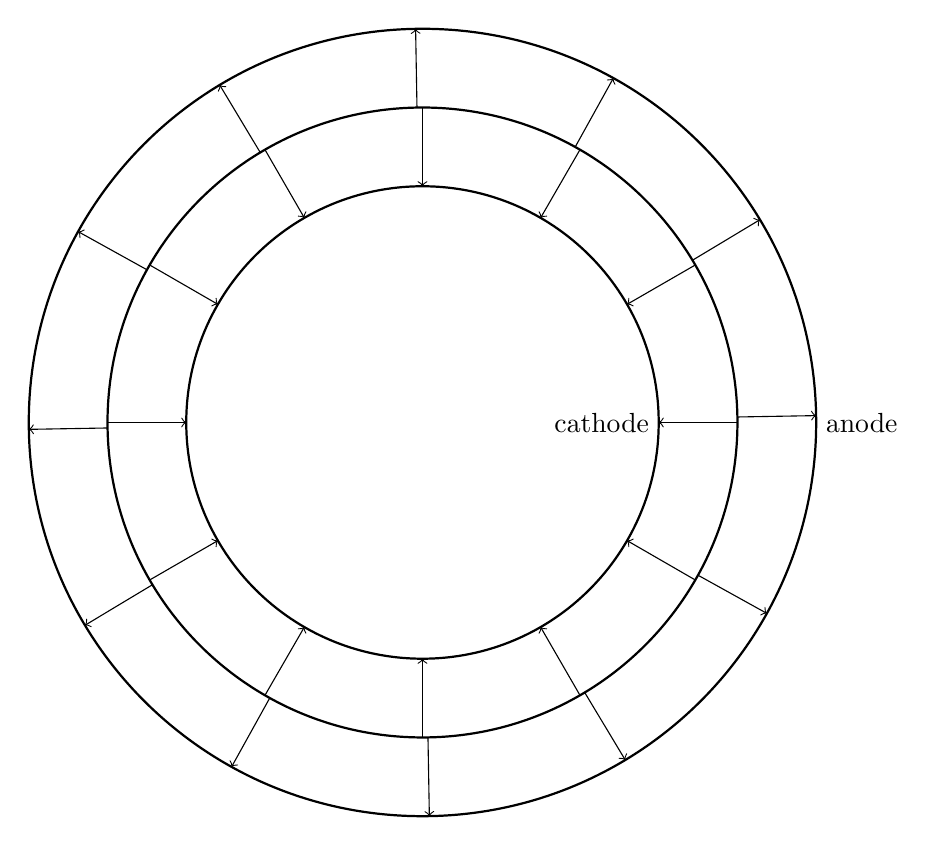
\begin{tikzpicture}
\draw[thick] (0, 0) circle (3);
\draw[thick] (0, 0) circle (4);
\draw[thick] (0, 0) circle (5);

\node[left] at (3,0) {cathode};
\node[right] at (5,0) {anode};

\foreach\x in {30, 60, 90, 120, 150, 180, 210, 240, 270, 300, 330, 360}
  {
  % gate is neutral and not blocking
  %\draw[<-] (\x:3) -- (\x:4);
  %\draw[<-] (\x:4) -- (\x:5);
  % gate is blocking
  \draw[<-] (\x:3) -- (\x:4);
  \draw[->] (\x+1:4) -- (\x+1:5);
  }

\end{tikzpicture}
\end{document}
